
\documentclass[11pt,a4paper]{article}

\usepackage[utf8]{inputenc}
\usepackage[T1]{fontenc}
\usepackage{lmodern}
\usepackage[margin=2.3cm]{geometry}
\usepackage{graphicx}
\usepackage{hyperref}
\usepackage{enumitem}
\usepackage{microtype}
\usepackage{parskip}
\usepackage{xcolor}
\usepackage{float}
\usepackage{subcaption}

% counter for questions
\newcounter{researchquestion}

% macro for questions
\newcommand{\researchquestion}[2]{%
    \refstepcounter{researchquestion}%
    \label{#1}%
    \par\medskip
    \noindent\textit{Q\theresearchquestion. #2}%
    \par\medskip
}

\setlength{\parindent}{0pt}
\setlength{\parskip}{5pt}

\hypersetup{
    colorlinks=true,
    linkcolor=black,
    urlcolor=blue,
    citecolor=black
}

\begin{document}

\begin{flushleft}
    {\LARGE\bfseries Sleep Monitoring Dashboard}\\[5pt]

    {\normalsize\textbf{Jakob Balkovec}}\\[3pt]
    {\small (840.073) Outcomes Research 26WS}\\
    {\small Medical University of Vienna}\\[6pt]
    {\small\color{gray} November 8, 2026}
\end{flushleft}

\vspace{0.3cm}

% --------------------------------------------------
\section{Motivation and Objective}
% --------------------------------------------------
\label{sec:motivation}

I have been an athlete for roughly 19 years. I started playing
golf when I was four years old and quickly progressed through
the junior ranks. Throughout middle school and high school,
I won several national and international titles, which
eventually helped me earn a scholarship to play NCAA Division I
golf at Seattle University.

Division I golf is extremely competitive and represents
the highest level of collegiate golf in the United States.
At that level, I quickly learned how much sleep, nutrition,
and mental preparation affected my performance, both on
and off the golf course.

Towards the end of my freshman year, I bought myself a
WHOOP band~\cite{whoop101}
(Figure~\ref{fig:whoop}). Initially, I just
wanted to see how well I was sleeping. Over time, however,
I became particularly interested in the journal feature
\cite{whoop2026journal}, which allowed me to record habits
and compare them with my sleep and recovery measurements. It gave me a better
idea of what seemed to help and what did not.

From that point on, I became quite interested in sleep.
I started reading research papers, attending workshops,
and paying more attention to my sleeping habits.
I do not necessarily enjoy sleeping more than the next
person, but I care about sleeping well and recovering
properly so that I can perform at my best. The importance of sleep for athletic performance and
recovery has also been discussed extensively in the
literature~\cite{walsh2021sleep}.

When I was tasked with designing a dashboard, sleep
monitoring was therefore the first thing that came to
mind. I wanted to approach the assignment from a
slightly different perspective: rather than creating
a dashboard for an athlete to track their own sleep,
I wanted to imagine that I was the researcher
conducting a sleep study.

% --------------------------------------------------
\section{Target Group and Dashboard Concept}
\label{sec:target}
% --------------------------------------------------

The intended users are clinicians, sports scientists,
and researchers monitoring sleep in athletes. For the
remainder of this report, let \textsc{CLRSH} denote the clinician,
researcher, or principal investigator using the dashboard.
The dashboards displayed previously collected data; no new study
was conducted.

The dashboard consists of two views. The first is an
overview of the entire study population
(Figure~\ref{fig:overview}). It is designed to give
\textsc{CLRSH} a quick summary of the collected measurements
without having to inspect each participant individually.

In particular, the overview should help answer
questions such as:

\researchquestion{q:average}{
    How much sleep are the athletes getting on average,
    and how many fall below seven hours?
}

\researchquestion{q:comparison}{
    Which athletes sleep the most or least, and are
    there noticeable differences across weekdays?
}

The second view, shown in Figure~\ref{fig:individual},
focuses on individual athletes and selected subgroups.
Here, \textsc{CLRSH} can examine sleep duration, variability,
and deviations from the selected average.

The dashboard also includes adjustable filters for
participants, weekdays, matchday categories, and
caffeine consumption. This makes it possible to
investigate more specific questions.

\researchquestion{q:caffeine}{
    How does sleep duration differ between observations
    with different reported levels of caffeine consumption?
}

\researchquestion{q:matchday}{
    Do athletes show different sleep patterns depending
    on the timing of a match?
}

These questions are exploratory. The dashboard is
intended to help identify patterns worth investigating,
rather than establish why those patterns occur.


% --------------------------------------------------
\section{Dataset Selection}
% --------------------------------------------------

I chose the REST study dataset~\cite{boeker2026rest}
because it was made publicly available post hoc,
after the study had already been completed.
The dataset was obtained from Zenodo~\cite{restdata2025} and was published in a form I could use directly. I did not change the source records, although some observations were excluded from particular calculations when the required values were missing.

The study followed 21 elite female football players over a period of 17 days. Data were collected using wearable devices (actigraphy), questionnaires, and other measurements related to sleep and daily habits. These included sleep duration, caffeine intake, screen time, soreness, and well-being. The dates were anonymized for privacy reasons.

I chose this dataset mainly because it contained both sleep measurements and information about habits that might influence sleep. This made it possible display the data where atheltes are treated like a group (filter by caffeine intake), but also compare individual athletes and examine differences under certain conditions (fitler by time-to-game-day).


% --------------------------------------------------
\section{Visualizations}
\label{sec:visualizations}
% --------------------------------------------------

\subsection*{Average Sleep by Athlete}

A horizontal bar chart was used to display the average sleep
duration for each athlete. I chose this visualization because
it made comparisons between athletes fairly straightforward.
The bars were sorted by sleep duration, making it easy to
identify which athletes slept the most and which slept the
least on average.

This was particularly useful in the overview dashboard,
where the goal was to get a quick understanding of the
entire group without looking at individual records.

\subsection*{Sleep Across the Week}

A heatmap was used to display sleep duration across different
weekdays. Each cell represented an average sleep duration,
with color indicating whether the value was relatively
high or low.

I chose a heatmap because it made it easier to spot patterns
across athletes and weekdays without having to compare a
large number of individual bars. It also allowed the user
to see whether certain athletes tended to sleep more or
less on particular days.

\subsection*{Sleep Duration Distribution}

A histogram was used to show the distribution of recorded
sleep durations. Rather than only displaying an average,
this visualization showed how frequently different sleep
durations occurred.

I included this because an average alone does not tell
the whole story. Two groups could have a similar average
sleep duration while having very different distributions.
The histogram made it easier to see where most observations
were concentrated and whether unusually short or long
sleep durations were present.

All three visualizations used previously collected data from the REST study.
The dashboards were descriptive and were not intended to establish cause and effect.

% --------------------------------------------------
\section{Software Selection}
\label{sec:software}
% --------------------------------------------------

I used Tableau Desktop for macOS~\cite{tableau2026} to build both dashboards.
The main reason for choosing Tableau was that Microsoft
Power BI does not run natively on macOS, and I did not
want to build the entire dashboard using Python.

Tableau allowed me to create calculated fields for the
individual KPIs, which were then displayed on the
dashboards. I also used it to create several charts
and graphs to better understand the data. Each
visualization was developed on a separate worksheet
before being combined into the final dashboards.

Another useful feature was the ability to add interactive
filters. These allowed users to select individual athletes,
filter observations by weekday, caffeine consumption,
and time relative to matchday, or adjust certain thresholds.
I also added navigation buttons to switch between the
overview and individual dashboards, making it easier
to move between the two without having to open separate
worksheets.

Working with Tableau was frustrating at times, particularly when
it came to formatting and configuring the dashboards. Still, I got
there in the end.


% --------------------------------------------------
\section{Limitations and Conclusion}
\label{sec:limitations}
% --------------------------------------------------

The biggest limitations were the small sample size
($n = 21$) and the relatively short observation period
($t = 17$ days). The analysis was descriptive rather
than causal, which made some of the variables I initially
found interesting difficult to interpret meaningfully.

Despite these limitations, the dashboards provided a
simple way to explore the available data, compare
athletes, and identify patterns that might be worth
investigating further.


% --------------------------------------------------
\section{Use of Generative AI}
\label{sec:ai}
% --------------------------------------------------

Generative AI (OpenAI ChatGPT, GPT-6) was used to assist with exploratory
data analysis, interpreting statistical measures, finding and understanding
Tableau documentation, troubleshooting Tableau and LaTeX, and editing the
wording and references in this report. The personal motivation and dashboard
work were my own. I retain responsibility for the analytical decisions,
verification of results, and the final dashboards.

% --------------------------------------------------
\section{References}
% --------------------------------------------------
\clearpage
\begin{thebibliography}{9}

\bibitem{boeker2026rest}
Boeker, M., Alexandersen, A., Thambawita, V.,
Midoglu, C., Johansen, D., Riegler, M. A.,
\& Halvorsen, P. (2026).
REST, Exploring Sleep Patterns and Influencing
Factors in Elite Female Football Athletes.
\textit{Scientific Data}, 13, Article 546.
\url{https://doi.org/10.1038/s41597-025-06331-8}

\bibitem{restdata2025}
Boeker, M., Thambawita, V., Riegler, M.,
\& Midoglu, C. (2025).
\textit{Exploring Sleep Patterns and Influencing
Factors in Elite Female Football Athletes}
(Version 4) [Dataset].
Zenodo.
\url{https://doi.org/10.5281/zenodo.16937033}

\bibitem{walsh2021sleep}
Walsh, N. P., Halson, S. L., Sargent, C.,
et al. (2021).
Sleep and the athlete: Narrative review and
2021 expert consensus recommendations.
\textit{British Journal of Sports Medicine},
55(7), 356--368.
\url{https://doi.org/10.1136/bjsports-2020-102025}

\bibitem{whoop2026journal}
WHOOP. (2026).
\textit{WHOOP Journal: How to Customize It
and See Behavior Impacts}.
\url{https://www.whoop.com/us/en/thelocker/the-whoop-journal/}
(Accessed: November 8, 2026).

\bibitem{whoop101}
WHOOP. (n.d.).
\textit{WHOOP 101}.
\url{https://developer.whoop.com/docs/whoop-101/}
(Accessed: November 8, 2026).

\bibitem{tableau2026}
Tableau. (n.d.).
\textit{Create a Dashboard}.
Tableau Desktop Documentation.
\url{https://help.tableau.com/current/pro/desktop/en-us/dashboards_create.htm}
(Accessed: November 8, 2026).

\bibitem{chatgpt2026}
OpenAI. (2026).
\textit{ChatGPT (GPT-6)} [Large language model].
\url{https://chatgpt.com/}

\bibitem{github2026}
Balkovec, J. (2026).
\textit{Outcomes Research Dashboard}.
GitHub Repository.
\url{https://github.com/j-balkovec/outcomes-research-dashboard}
(Accessed: November 8, 2026).

\end{thebibliography}

\clearpage
\appendix
\section{Supplementary Figures}

% whoop

\begin{figure}[H]
    \centering

    \begin{subfigure}[t]{0.45\textwidth}
        \centering
        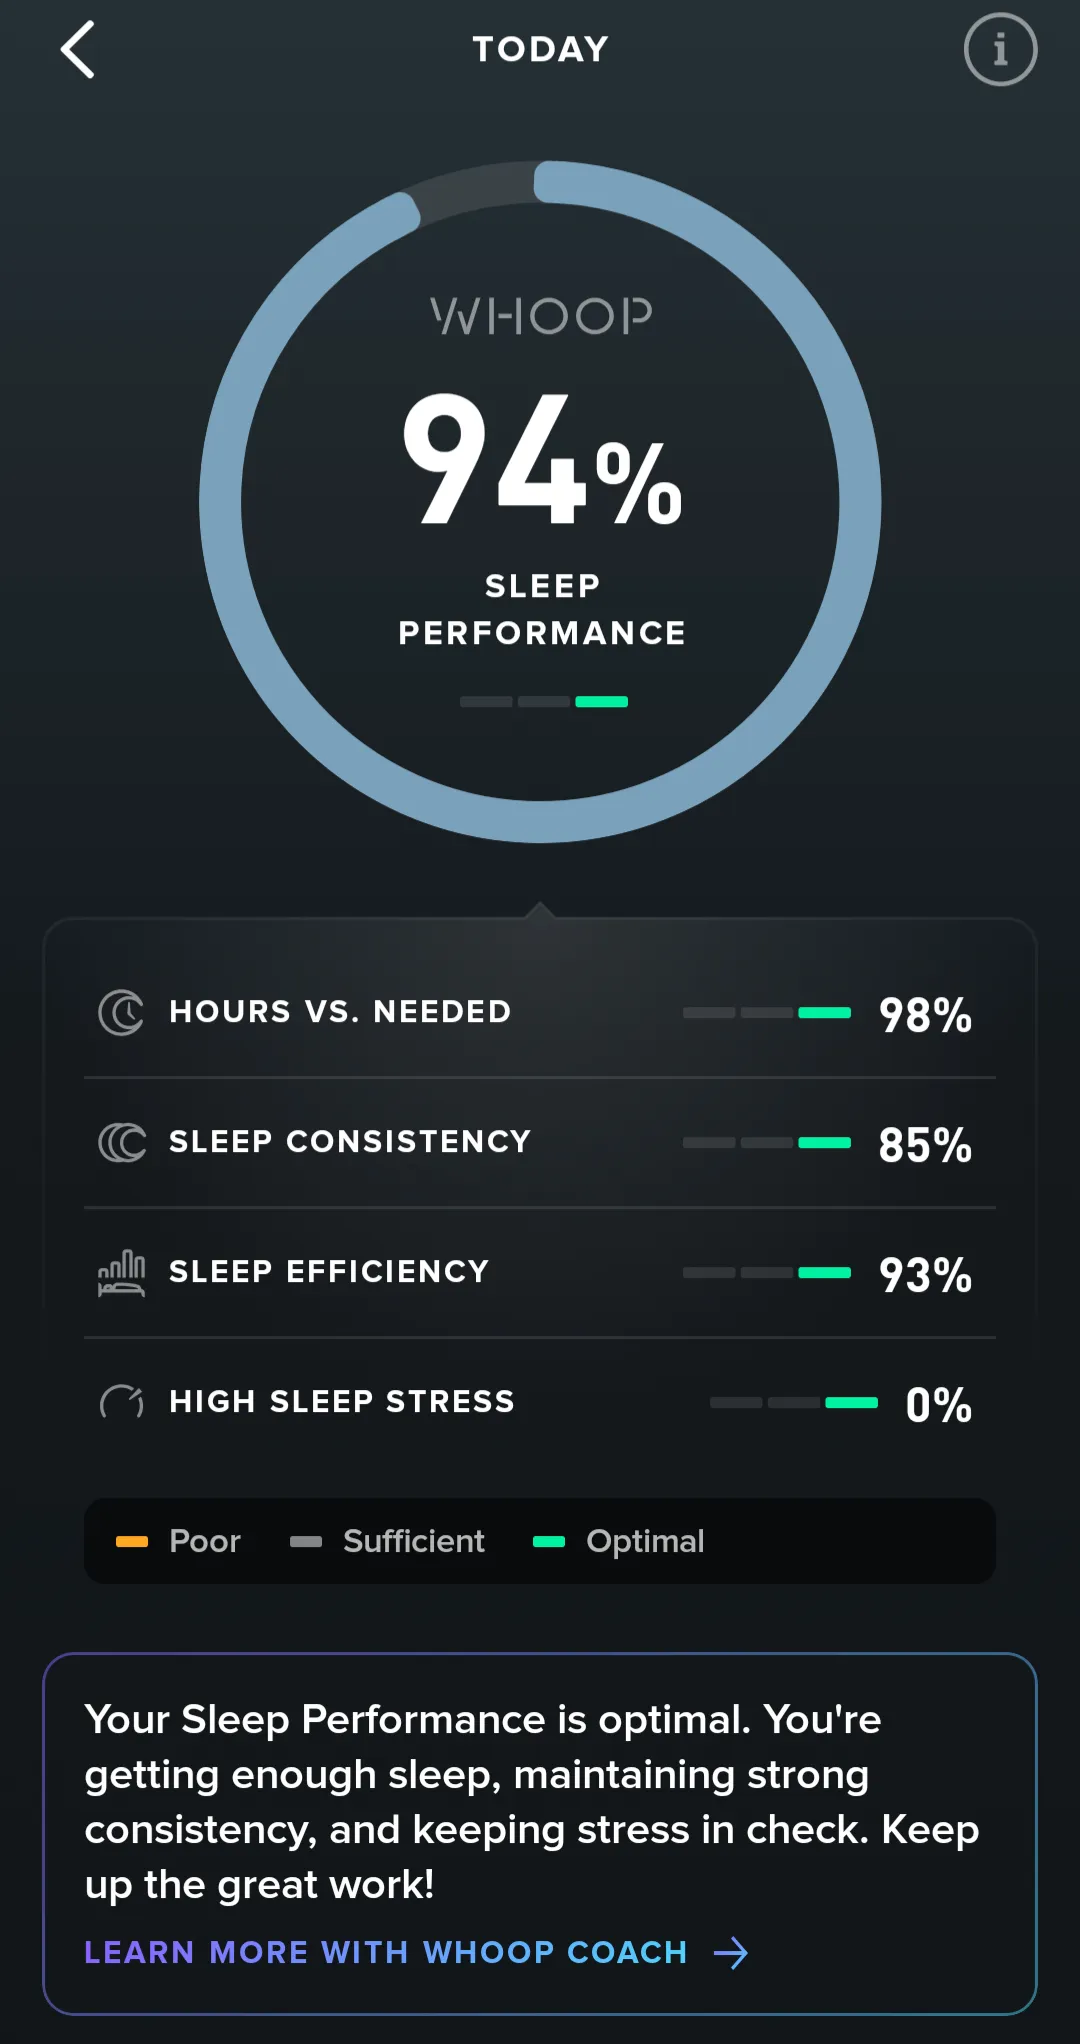
\includegraphics[
            width=\linewidth,
            height=6cm,
            keepaspectratio
        ]{img/WhoopSleep.png}
        \caption{Sleep overview}
        \label{fig:whoop-sleep}
    \end{subfigure}
    \hfill
    \begin{subfigure}[t]{0.45\textwidth}
        \centering
        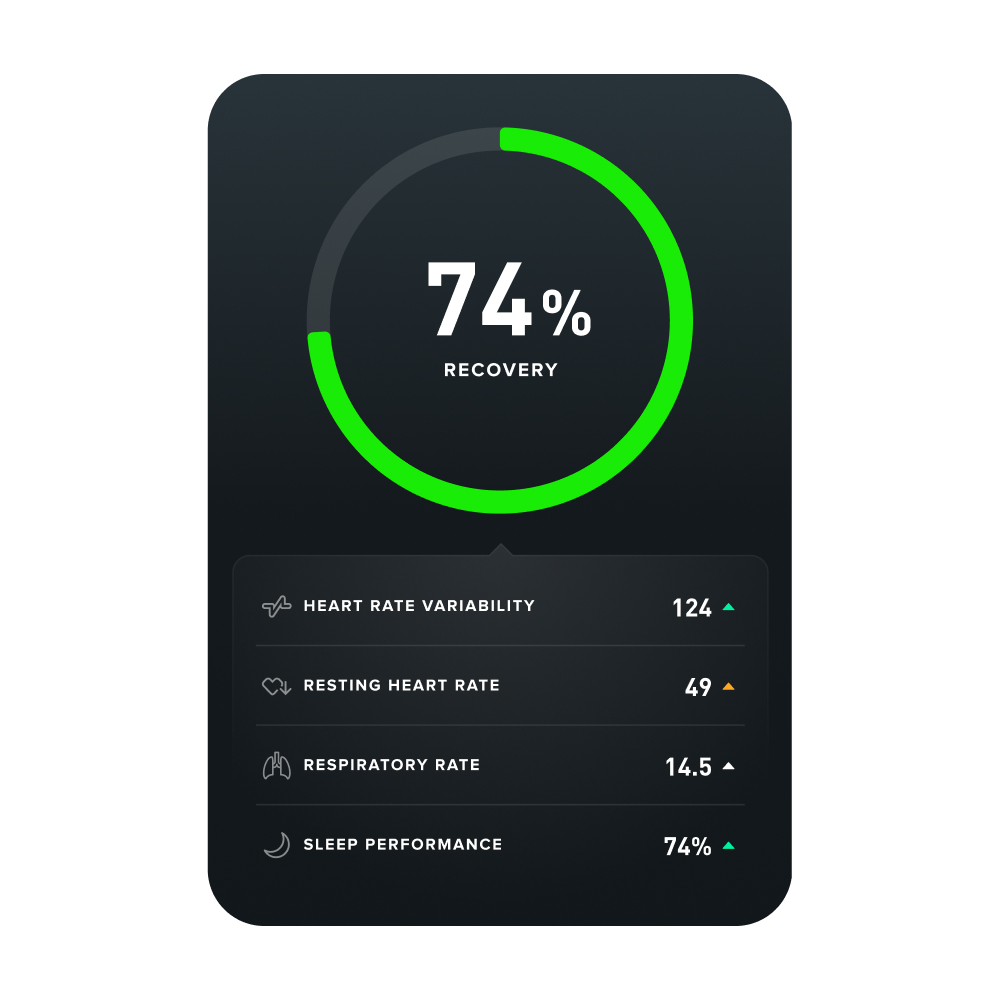
\includegraphics[
            width=\linewidth,
            height=6cm,
            keepaspectratio
        ]{img/WhoopRecovery.jpg}
        \caption{Recovery metrics}
        \label{fig:whoop-recovery}
    \end{subfigure}

    \par\vspace{0.4cm}

    \begin{subfigure}[t]{0.45\textwidth}
        \centering
        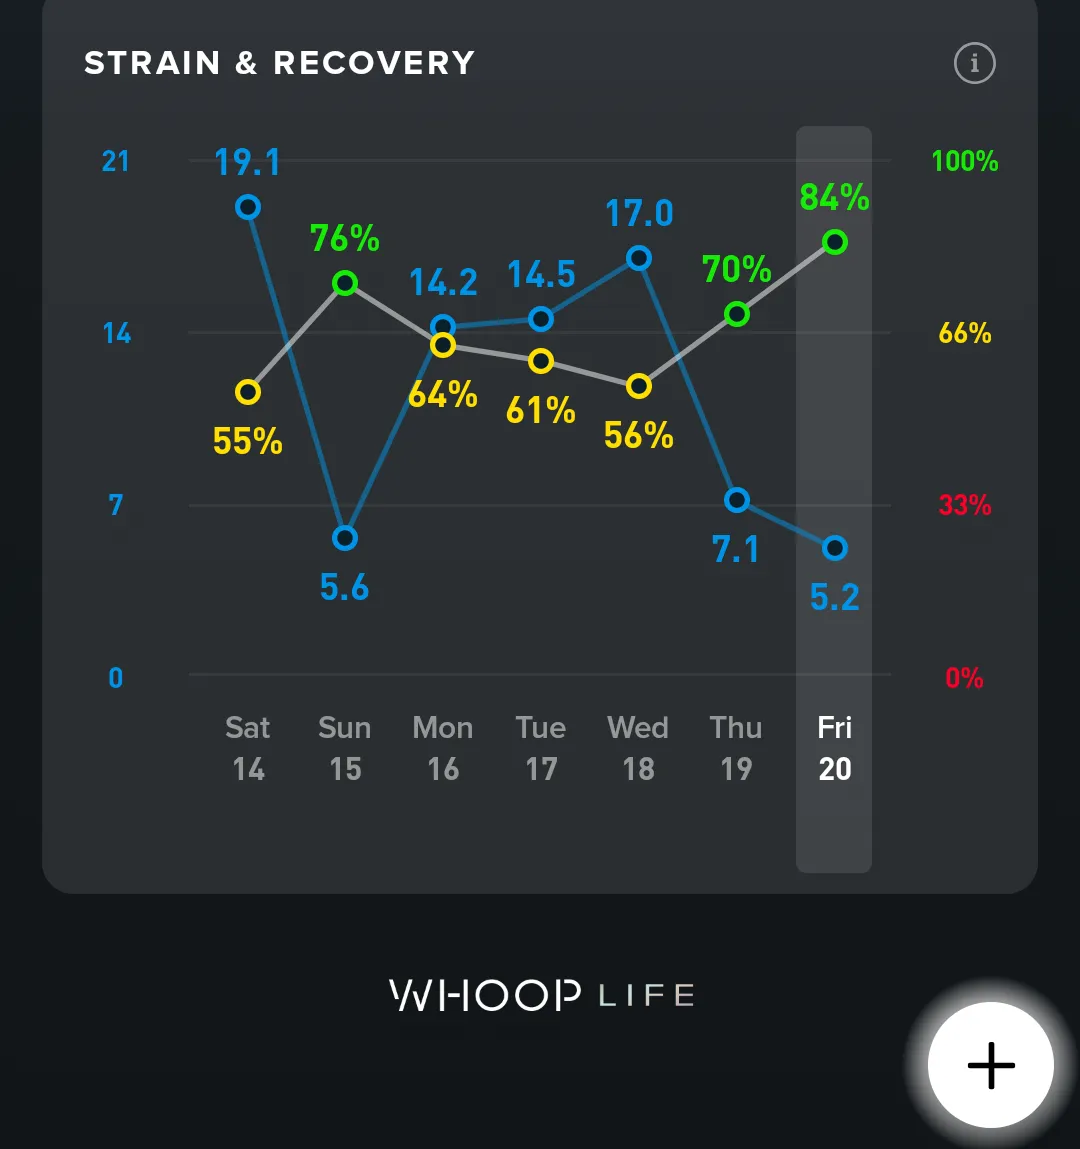
\includegraphics[
            width=\linewidth,
            height=6cm,
            keepaspectratio
        ]{img/WhoopStrain.png}
        \caption{Strain monitoring}
        \label{fig:whoop-strain}
    \end{subfigure}
    \hfill
    \begin{subfigure}[t]{0.45\textwidth}
        \centering
        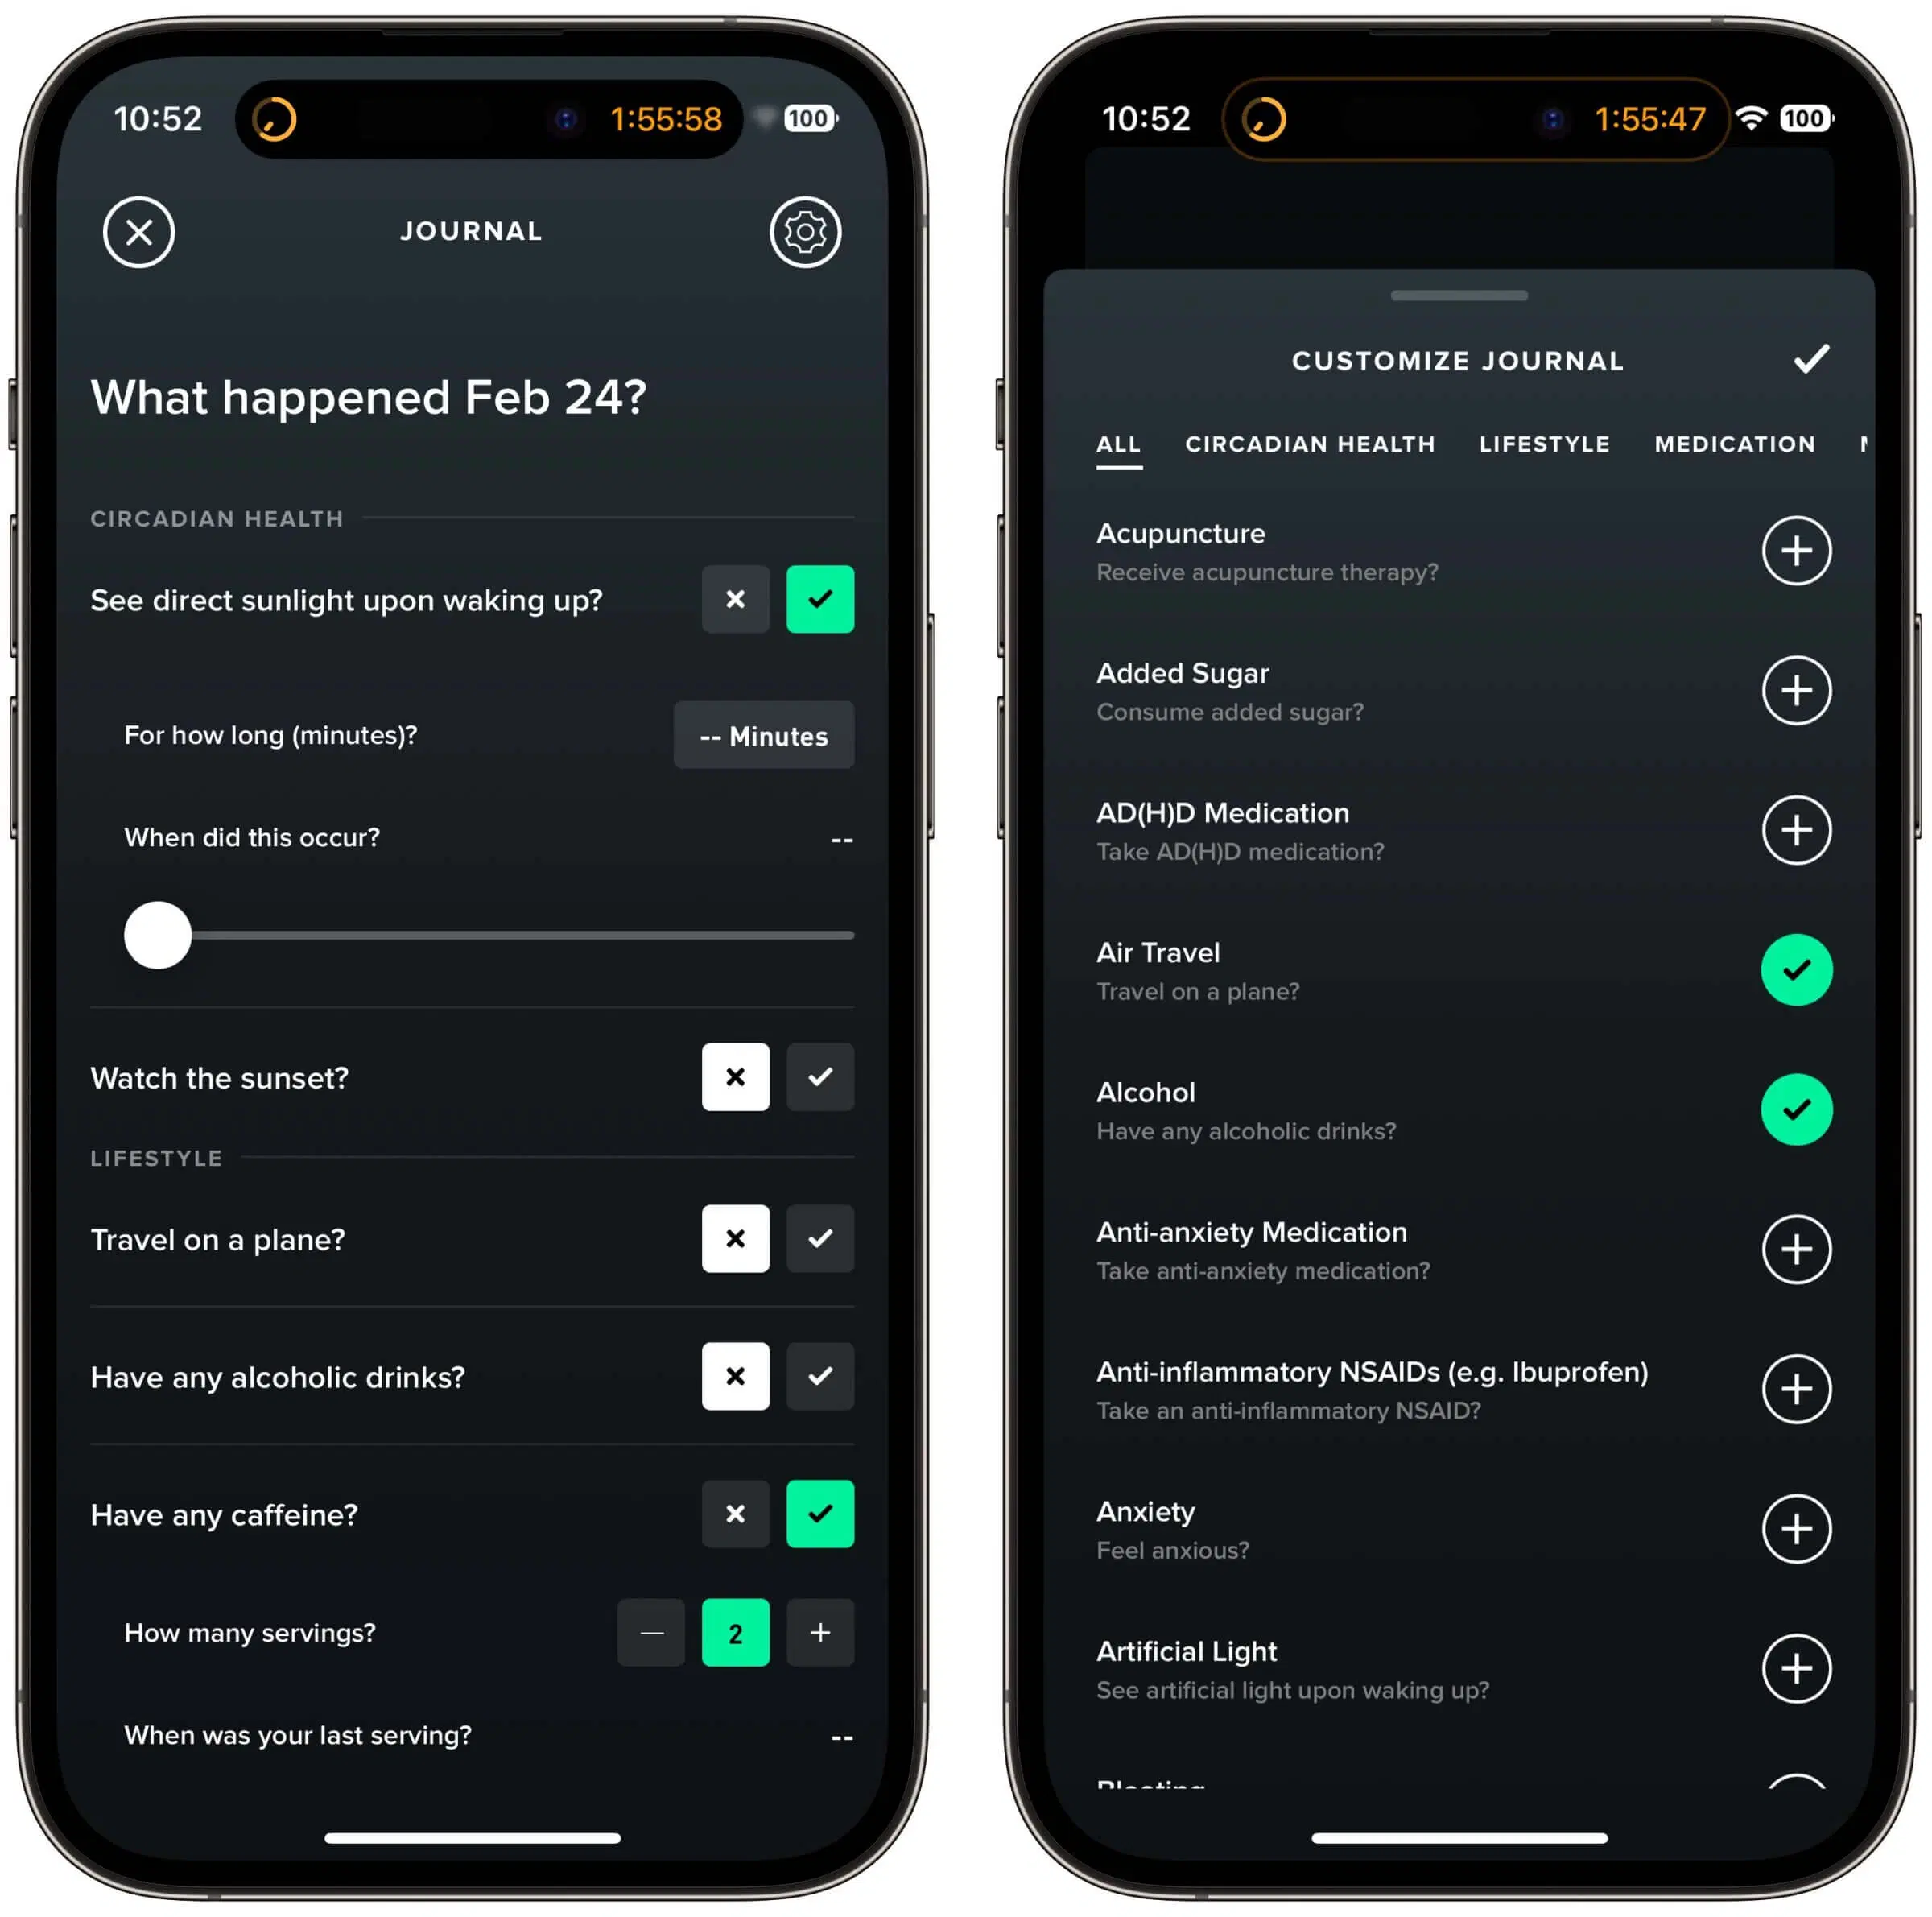
\includegraphics[
            width=\linewidth,
            height=6cm,
            keepaspectratio
        ]{img/WhoopJournal.png}
        \caption{Journal}
        \label{fig:whoop-journal}
    \end{subfigure}

    \caption{
        WHOOP monitoring features, including sleep,
        recovery, strain, and the journal.
        Source: WHOOP app screenshots (see \cite{whoop101,whoop2026journal}).
    }
    \label{fig:whoop}
\end{figure}

% overview

\begin{figure}[H]
    \centering
    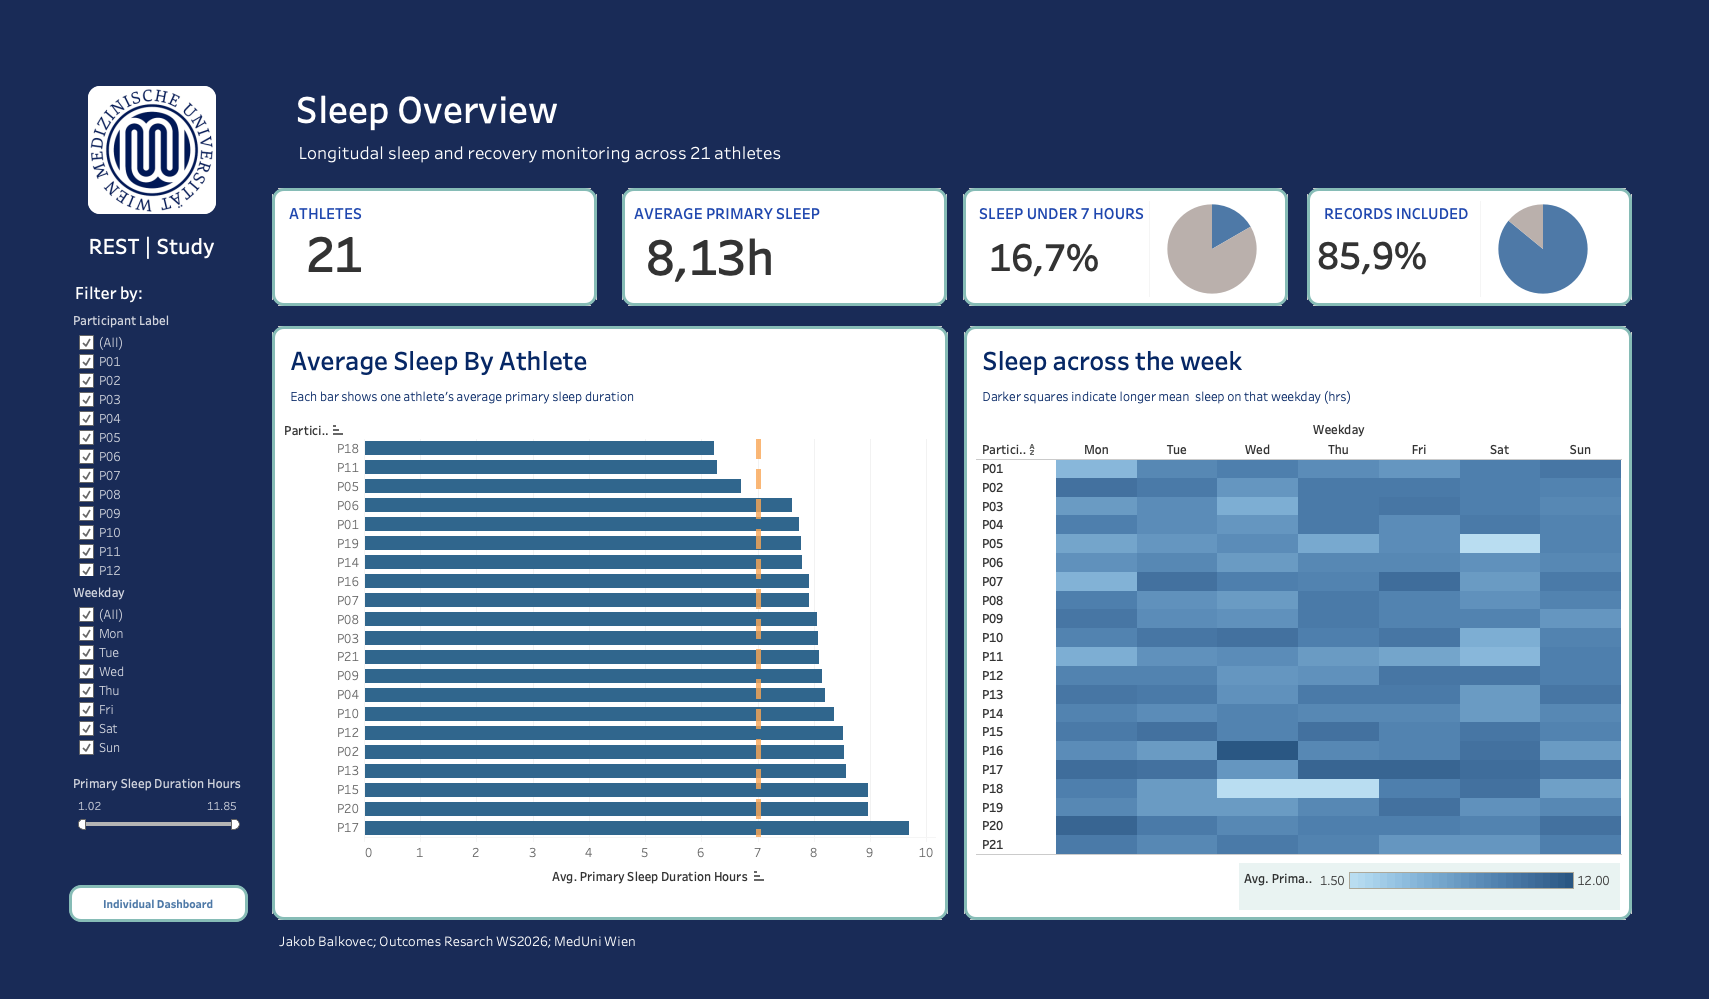
\includegraphics[
        width=\textwidth,
        keepaspectratio
    ]{img/SleepOverview.png}

    \caption{
        Sleep Overview dashboard displaying study-level
        measurements, participant comparisons, and
        weekday sleep patterns. Author's own Tableau dashboard.
    }
    \label{fig:overview}
\end{figure}

% individual

\begin{figure}[H]
    \centering
    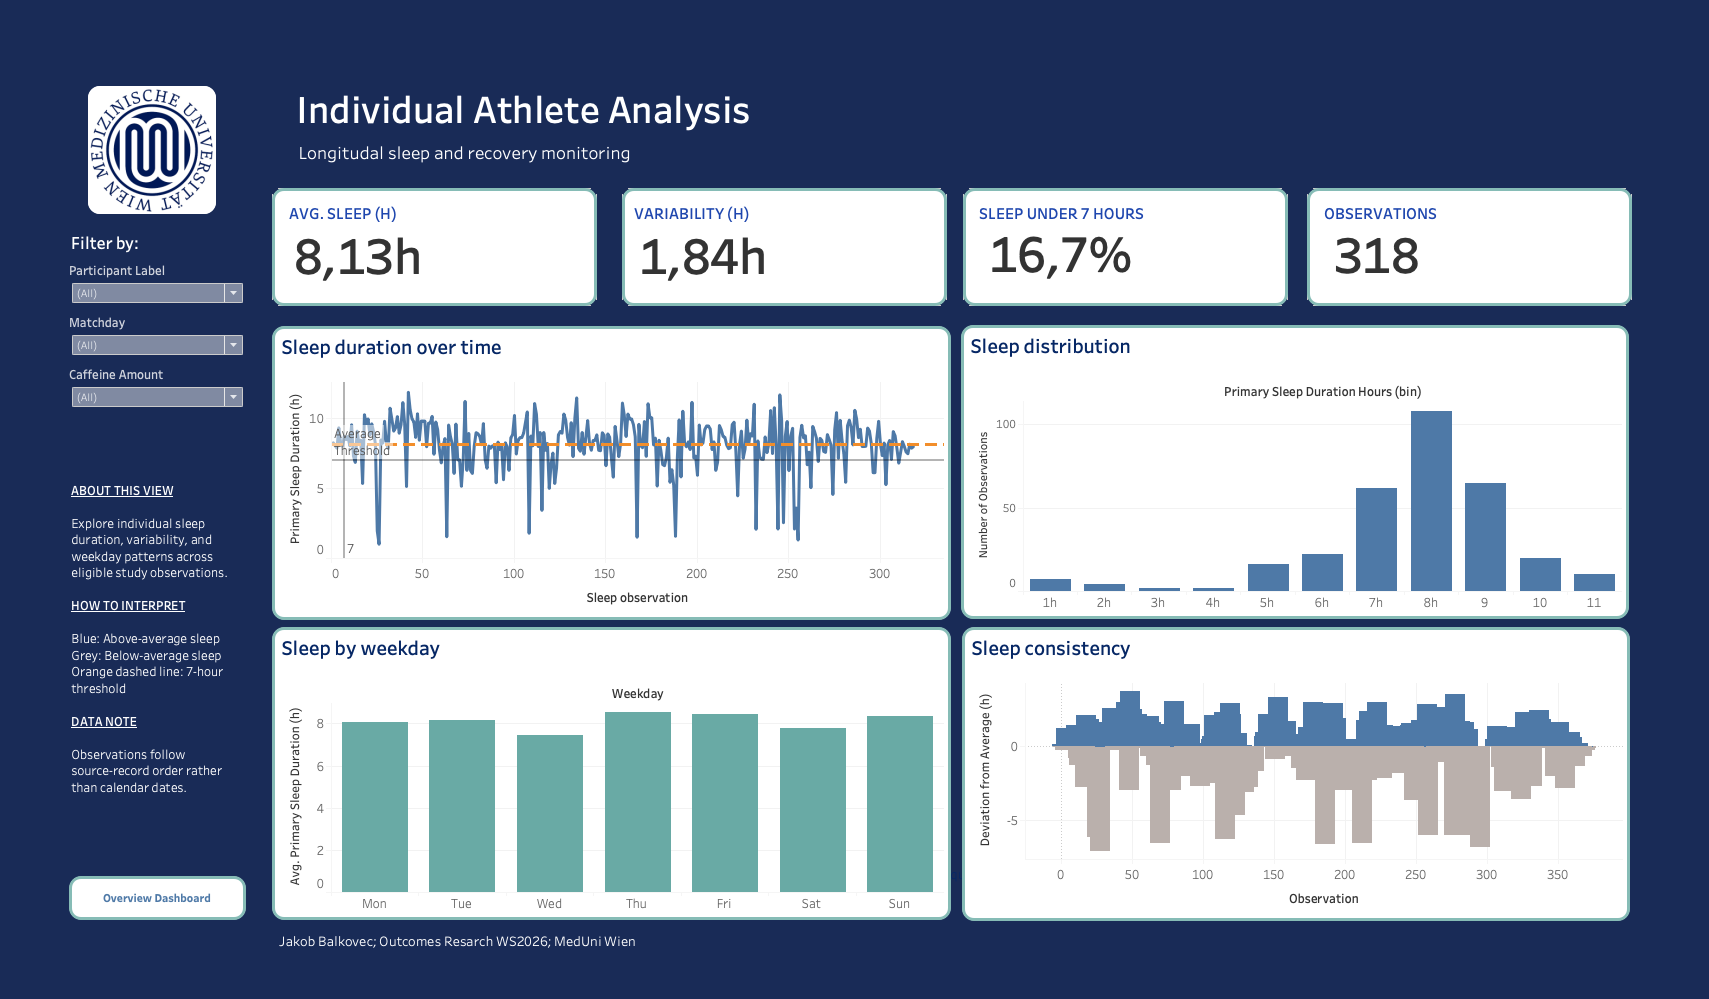
\includegraphics[
        width=\textwidth,
        keepaspectratio
    ]{img/IndividualDashboard.png}

    \caption{
        Individual Athlete Analysis dashboard showing
        sleep distributions, variability, and
        participant-level filtering. Author's own Tableau dashboard.
    }
    \label{fig:individual}
\end{figure}

\end{document}
% Jakob Balkovec, Nov 8th 2026

